\documentclass{standalone}

\usepackage{verbatim}
\usepackage{pst-circ}

\usepackage{pgfplots}
\usepgfplotslibrary{polar}
\pgfplotsset{compat=1.10}

\pgfplotsset{mypolarplot/.style={%
  clip=false, 
  domain=0:360,
  samples=180,
  grid=both, 
  major grid style={black}, 
  minor x tick num=5,
  minor y tick num=1,
  xtick={0,30, 45 ,60, 90, 120,135, 150, 180, 210, 225, 240, 270, 300, 315, 330},
  xticklabels={%
    $0$,
    $\frac{ \pi}{6}$,
    $\frac{ \pi}{4}$,
    $\frac{ \pi}{3}$,
    $\frac{ \pi}{2}$,
    $\frac{2\pi}{3}$,
    $\frac{3\pi}{4}$,
    $\frac{5\pi}{6}$,
    $\pi$,
    $\frac{7\pi}{6}$,
    $\frac{5\pi}{4}$,
    $\frac{4\pi}{3}$,
    $\frac{3\pi}{2}$,
    $\frac{5\pi}{3}$,
    $\frac{7\pi}{4}$,
    $\frac{11\pi}{6}$
  },
  yticklabel style={anchor=north}, 
}}

\begin{document}
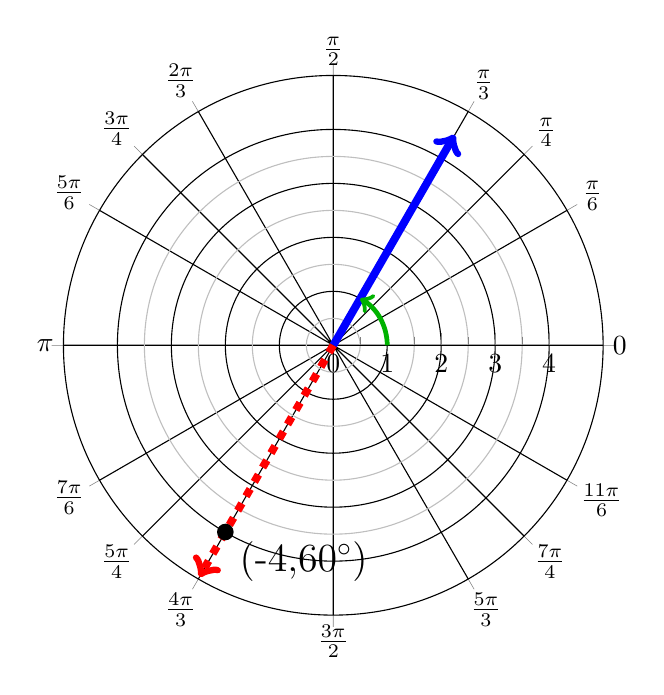
\begin{tikzpicture}
\begin{polaraxis}[%
  ymax=5,
  ytick={0,1,2,3,4},
  mypolarplot,
]

\draw [line width=1mm, blue,  -> ] (0, 0) -- (225, 390 ) ;
\draw [line width=1mm, red, dashed,  -> ] (0, 0) -- (-248, -429 ) ;
\fill  (-200, -346) circle (3 pt) ;

\draw (-55, -400) node {\Large (-4,$60^\circ $) } ;
\draw [line width=.6mm, -> , green!70!black ] (100, 0) arc (0:60:100);

\end{polaraxis}
\end{tikzpicture}
\end{document}